\chapter{Experimental reach}
\label{chap:reach}

\section{Proposed Measurements}

We propose to measure the semi-inclusive deep-inelastic scattering off  $^2$H and $^4$He by tagging a low momentum recoiling spectator ($P_{A-1}<300$ MeV/$c$). The reactions we are going to study are:
\begin{itemize}
\item $^2$H$(e, e' p)X$ --- bound neutron;
%\item $^3$He$(e, e' d)X$ --- bound proton;
\item $^4$He$(e, e'~^3\mathrm{H})X$ --- bound proton;
\item $^4$He$(e, e'~^3\mathrm{He})X$ --- bound neutron;
\end{itemize}
 
The semi-inclusive cross section $\sigma_1^A$ for each target will be measured. The $\vec P_{A-1}$ dependence of the cross section ratio on different targets, $R(A,A',|\vec P_{A-1}|)$, as defined in Eq.~\ref{eq:ratio} will be used to test the spectator mechanism in the first place. We are going to measure the ratio $R(\mathrm{D},^4\mathrm{He})$ for scattering from a bound neutron and proton, respectively.

The dependence of the semi-inclusive cross section on $x$ and $\vec P_{A-1}$ will be accessed. Specifically, the ratio of the cross section at different $x$, $R^A$, as defined in Eq.~\ref{eq:ratio_a} and the semi-inclusive EMC ratio $R_0 (x,Q^2)$ in Eq.~\ref{eq:semi_emc} will be extracted and directly compared to various EMC models.

The bound structure function $F_2^{n/p}$ in different nuclear targets will be extracted from these measurements. The comparison between $(F_2^{p})^{bound}$ in $^4$He and $(F_2^p)^{free}$ can be used as a benchmark for the treatment of the nuclear effect in extracting the free neutron structure function from the deuterium data. In addition, by detecting the processes $^4$He$(e,e'^3\mathrm{H)}$ and $^4$He$(e,e'^3\mathrm{He})$ simultaneously, we can measure the bound proton/neutron structure function ratio $(F_2^n/F_2^p)^{bound}$ in $^4$He which is a compact system with large nuclear effect. It allows us to extract the distributions of $d/u$ for the bound nucleon, and investigate the isospin dependence of the anti-shadowing and EMC effects~\cite{Brodsky:2004qa,Cloet2009}.

\subsection{Detector Performance Studies}

To estimate the rates, we developed a Monte-Carlo simulation based on PYTHIA with some basic nuclear effects. The interaction is generated in the impulse approximation. We simulate the Fermi motion of the nucleons in the target nuclei according to the distribution provided by AV18+UIX potentials~\cite{Wiringa1995,Pudliner1997,Wiringa}, this lead to a target nucleon with a momentum $\vec p_n$. The nuclear spectator is generated with a kinematic opposite to the interacting nucleon, -$\vec p_n$. The PYTHIA Monte-Carlo provides simulation for the DIS interaction and the fragmentation of the partons, in which no nuclear effect is included.

The generated final-state particles go through acceptance tests. Electrons, which will be detected by the forward detector, are treated by the fast Monte Carlo of the CLAS12. The recoiling nuclei (including protons) detection has a different set of constraints based on the acceptance determined in the simulation described in section~\ref{sec:sim} and represented in Fig.~\ref{fig:acceptance}. On top of these estimates, we apply an overall 75\% efficiency to this detection setting to account for the fiducial cuts and detector inefficiencies.

\subsection{Projections}

\begin{figure}[tbp]
  \begin{center}
    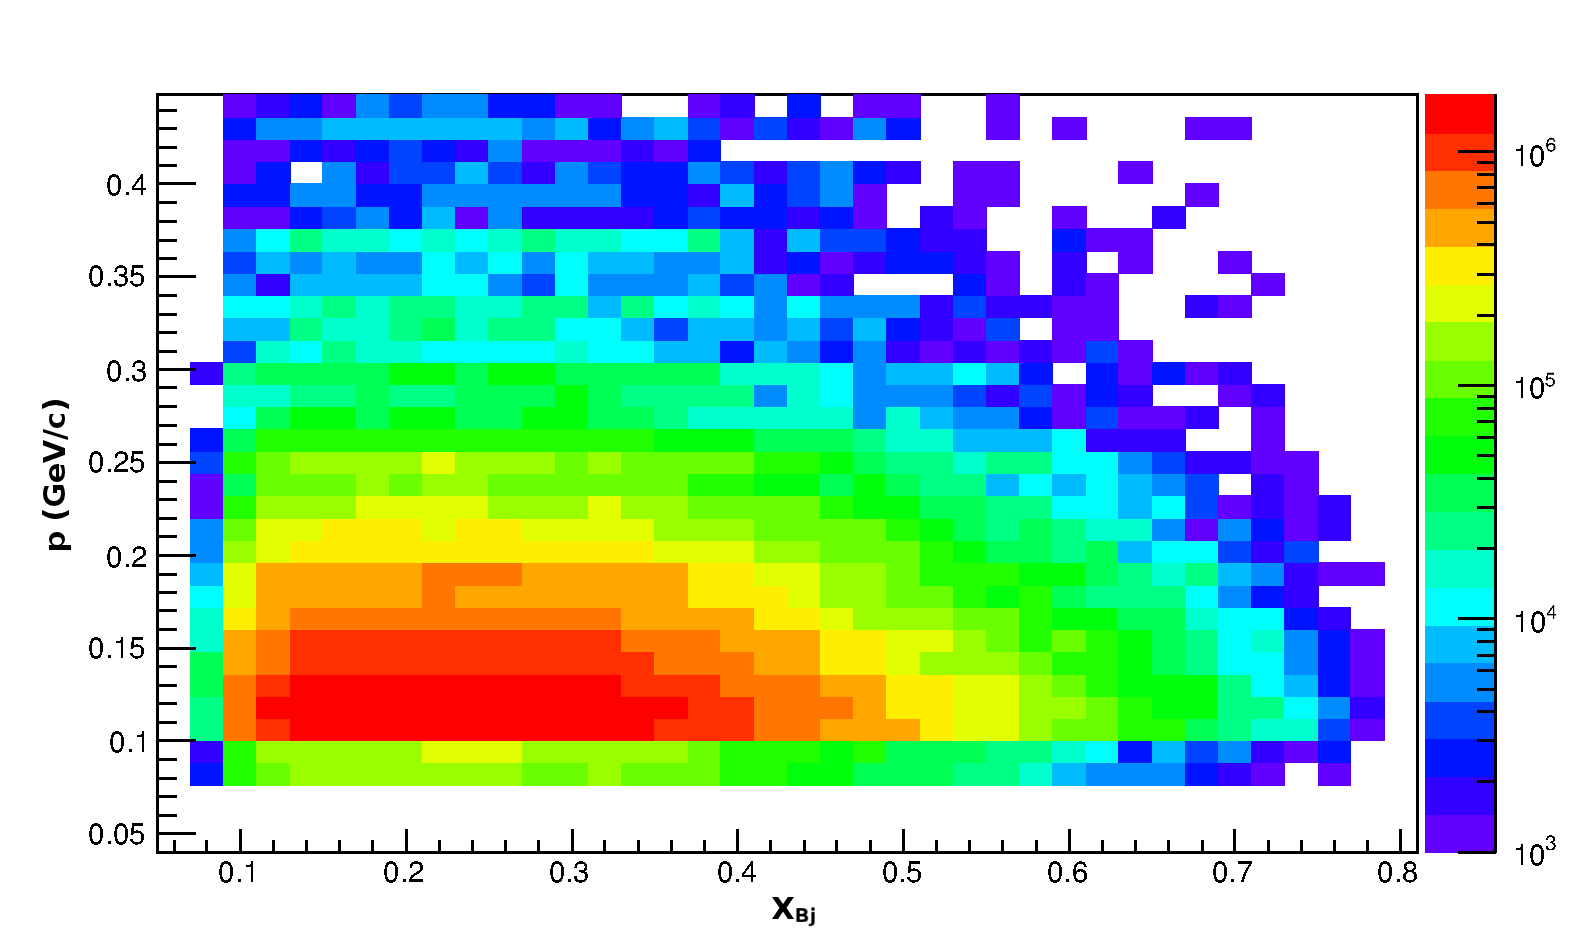
\includegraphics[angle=0, width=0.65\textwidth]{./fig-chap3/MomVsX-H3}
    \caption{Expected event count as a function of $x_B$ and the recoil momentum of the $^3$H from a $^4$He target.}
    \label{fig:xb_vs_p}
  \end{center}
\end{figure}

The error bars and counts presented in the following figures were evaluated assuming 60 days of beam time (30 on $^2$H and 30 on $^4$He). Based on our simulation, we determine the available kinematic range and production rates accessible. The $x_B$ and recoil momenta distributions are illustrated in Fig.~\ref{fig:xb_vs_p} for tagged $^3H$ out of an $^4$He target, this illustrates the available phase space for a measurement of the bound proton structure function. 

\subsubsection{Testing the Spectator Model}

\begin{figure}[tbp]
  \begin{center}
    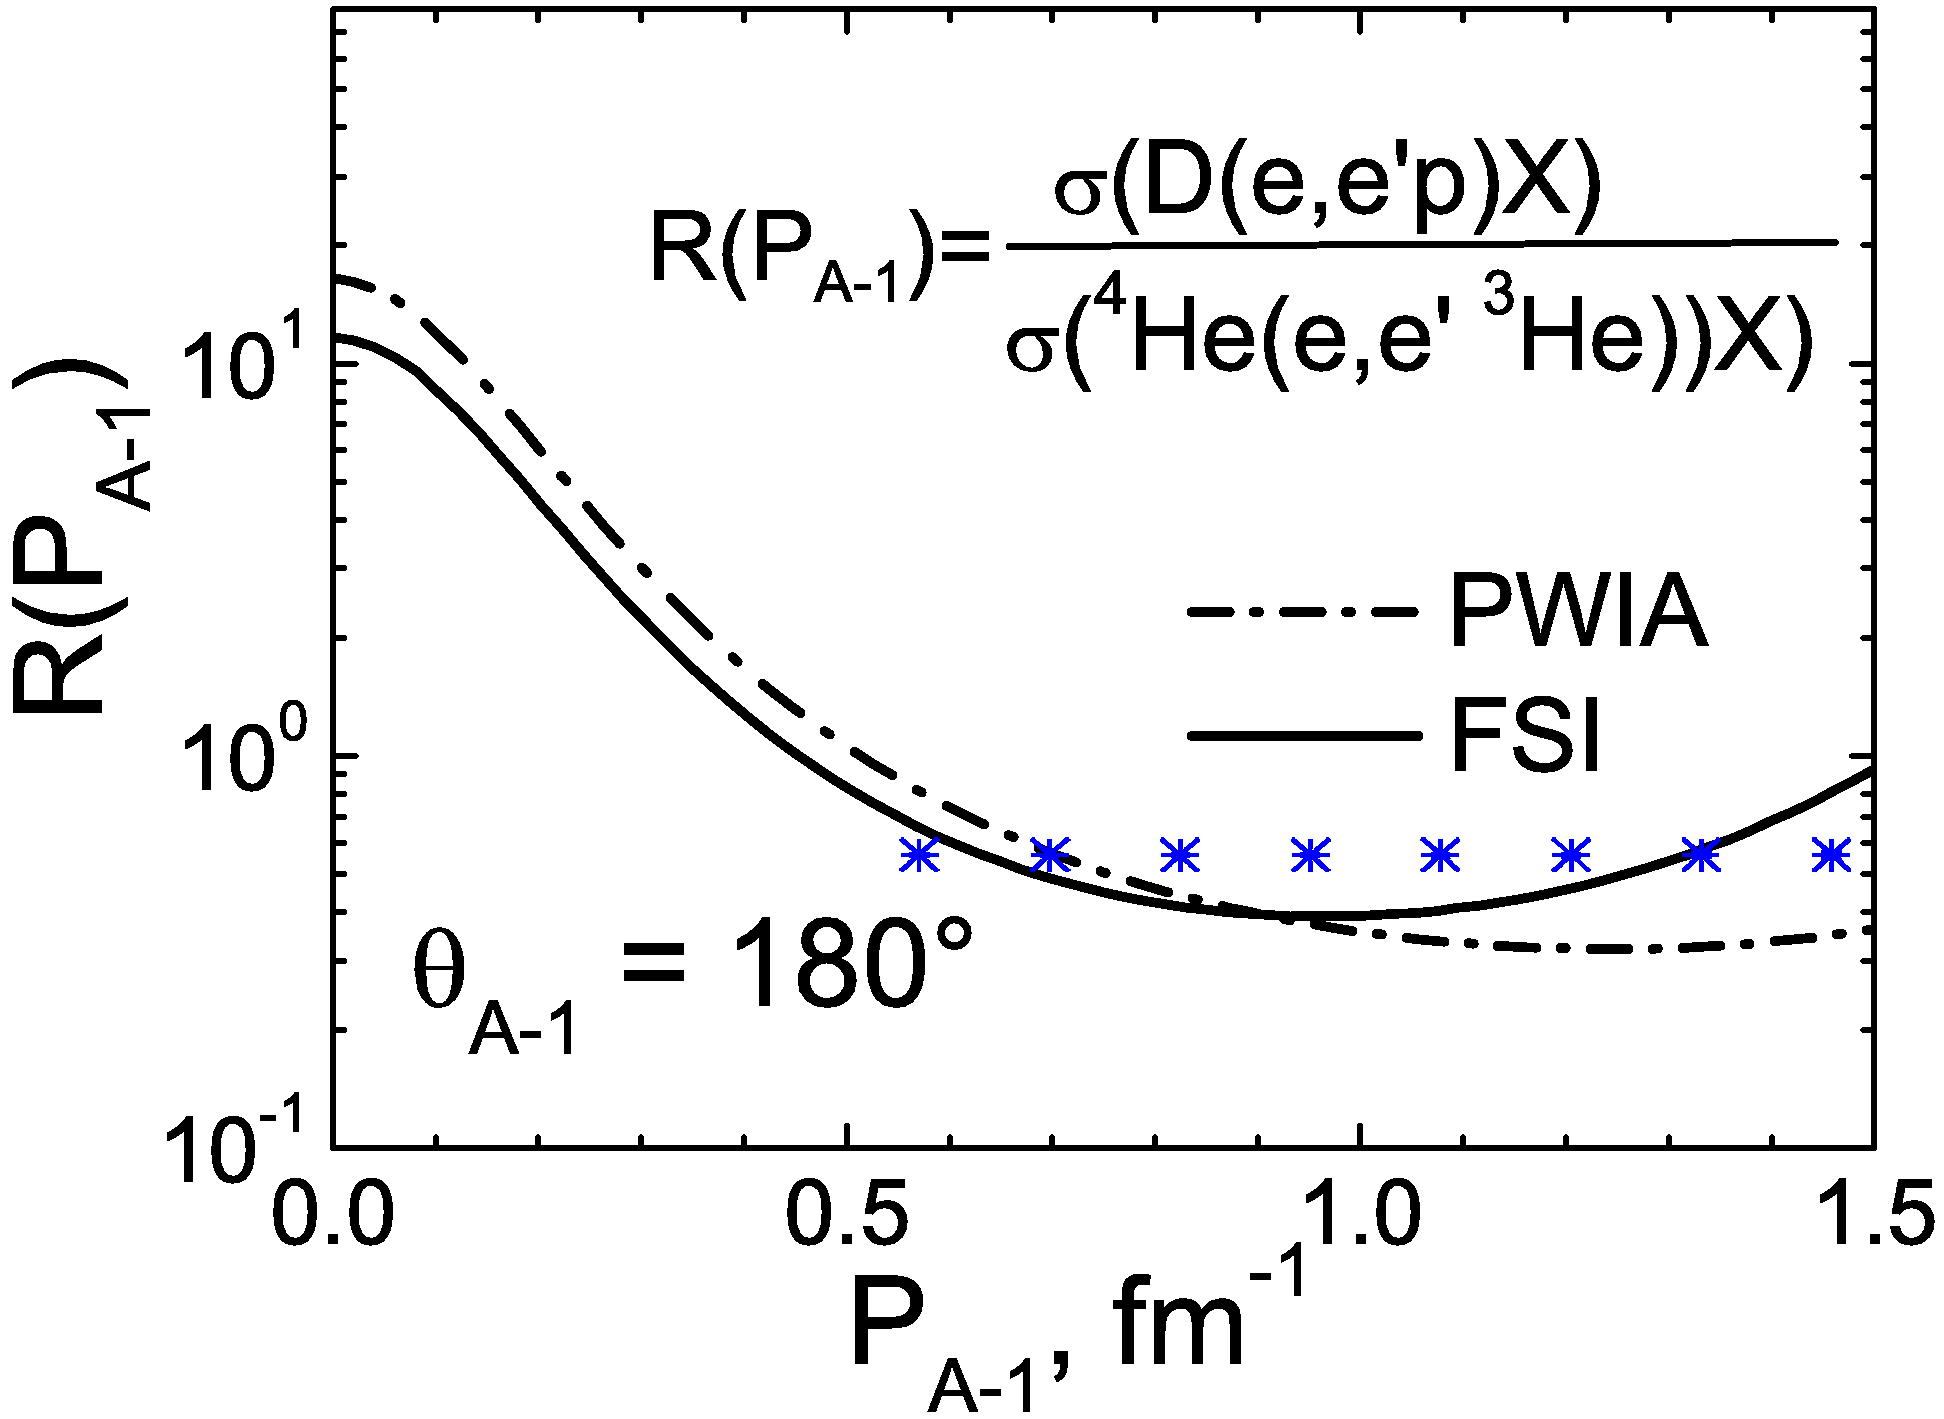
\includegraphics[angle=0, width=0.56\textwidth]{./fig-chap3/Ratio_He4}
    \caption{This figure is similar to figure \ref{fig:ratio_spec}, it shows the predictions for CLAS12 kinematic~\cite{CiofidegliAtti1999,CiofidegliAtti2012} of the ratio $R(^4$He$,^2$H$,|\vec P_{A-1}|)$ compared to projected statistical error bars for the proposed experiment (blue points).}
    \label{fig:ratio_spec_proj}
  \end{center}
\end{figure}

The projections presented in Fig.~\ref{fig:ratio_spec_proj} show the capability of this experiment to measure cross section ratios of DIS on a bound nucleon in various light nuclei and, therefore, our capability to check the validity of the spectator model used by the theoretical predictions. Statistical error bars in this figure are very modest making evident our capability to test the spectator model in detail. The high precision we can obtain for this channel should also lead to valuable confirmation of assumptions made for other similar measurements, such as BoNuS.

\subsubsection{Testing the Rescaling Models}

\begin{figure}[tbp]
  \begin{center}
    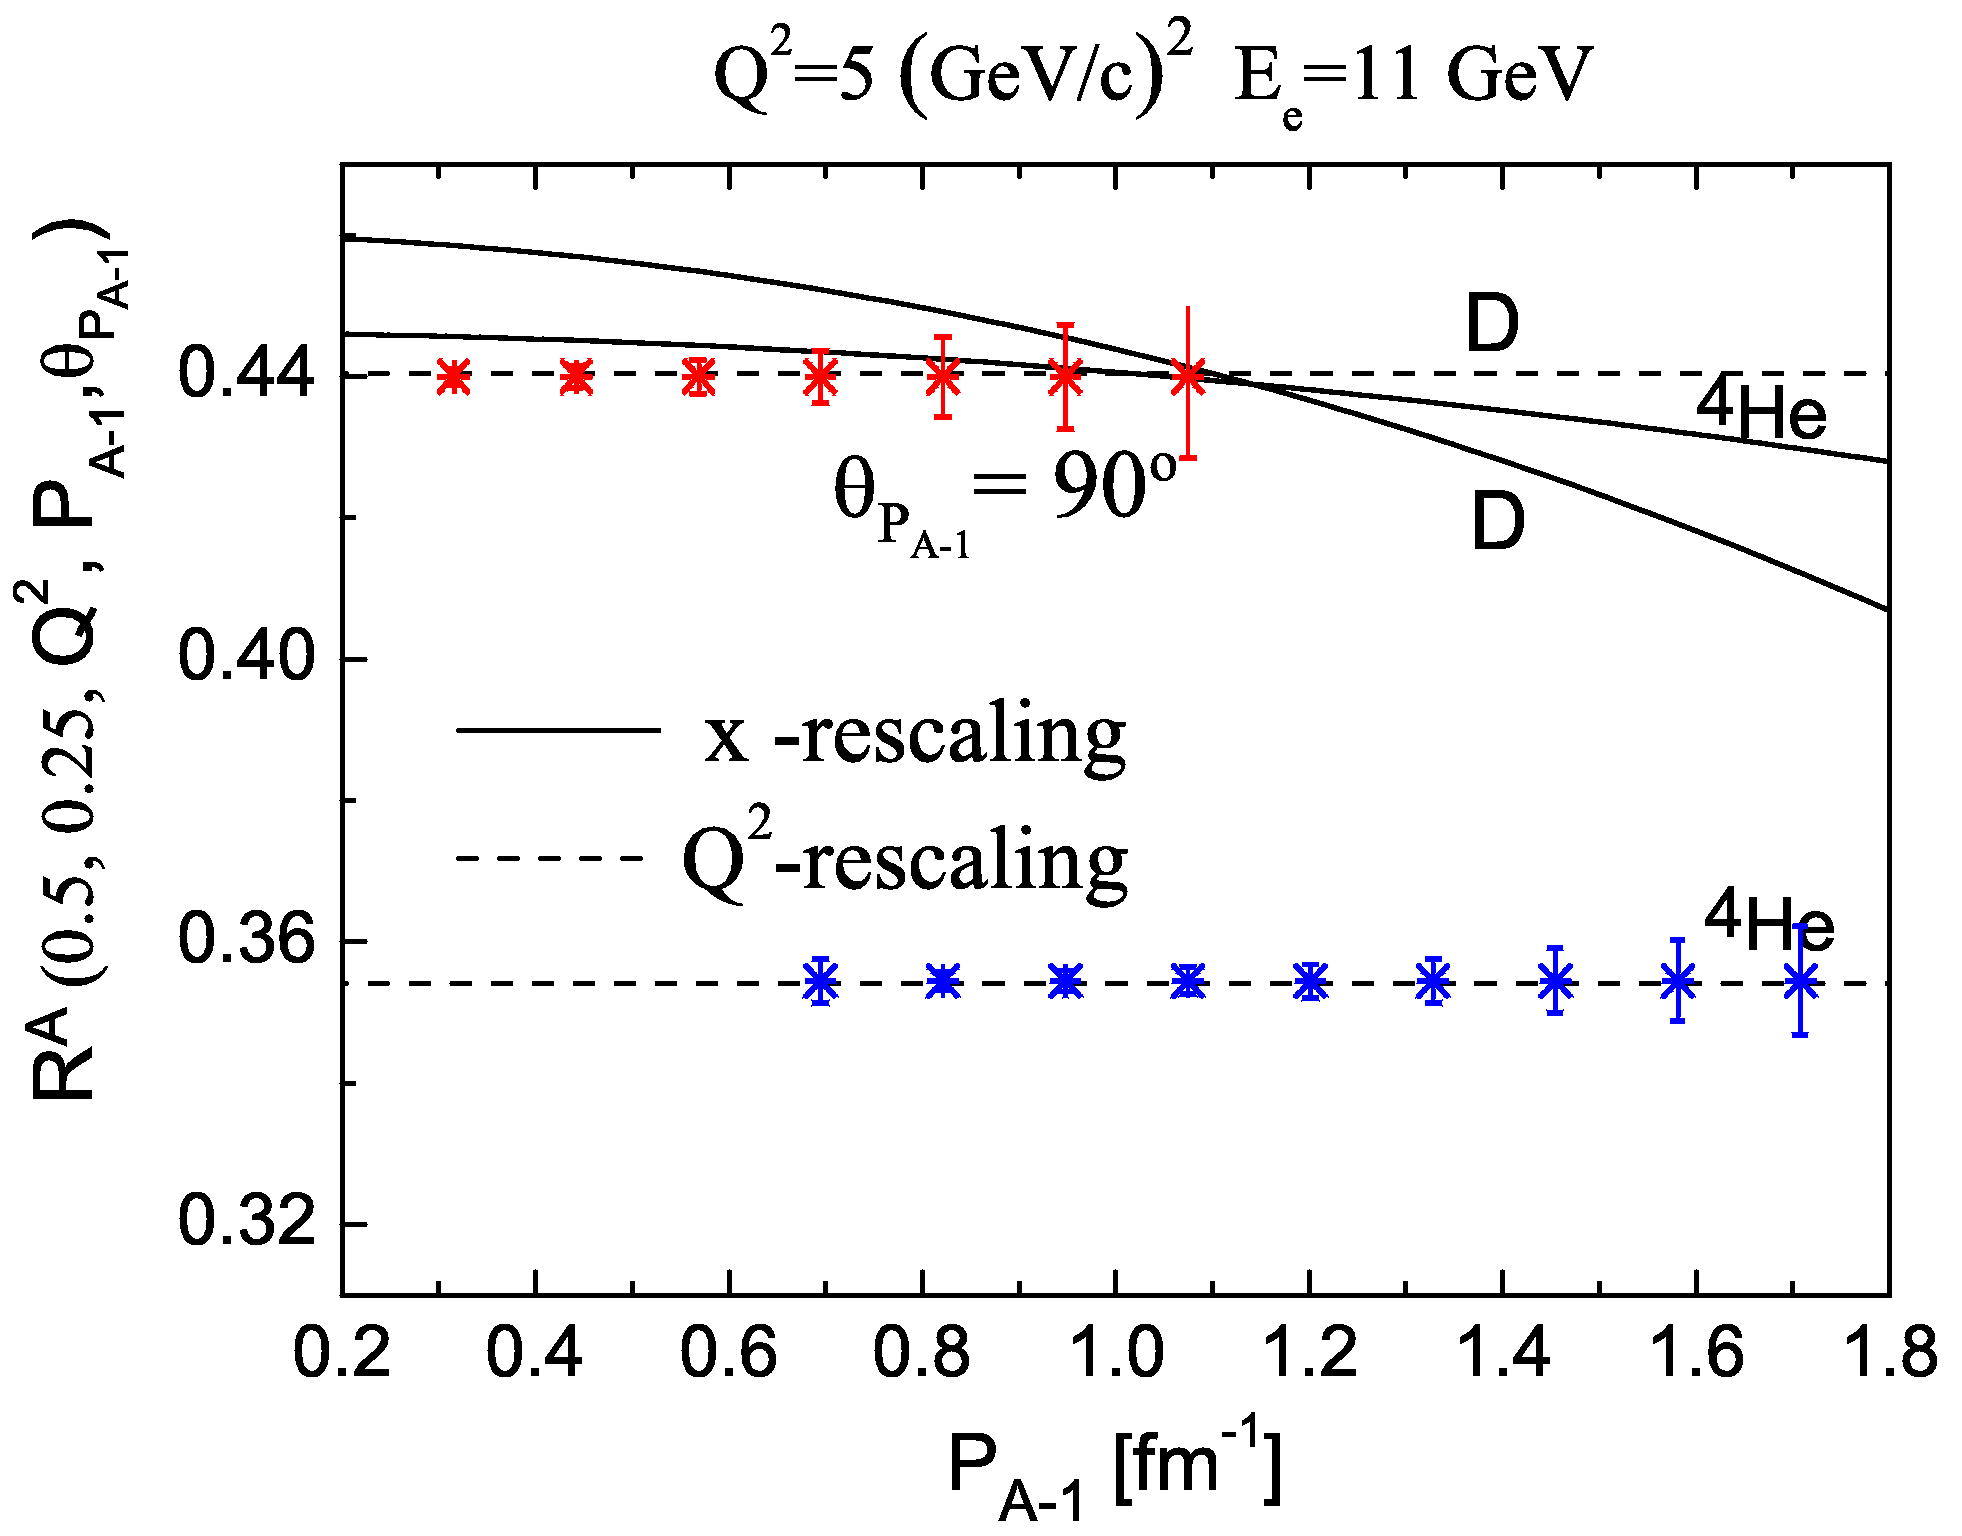
\includegraphics[angle=0, width=0.47\textwidth]{./fig-chap3/Fig5New_90}
    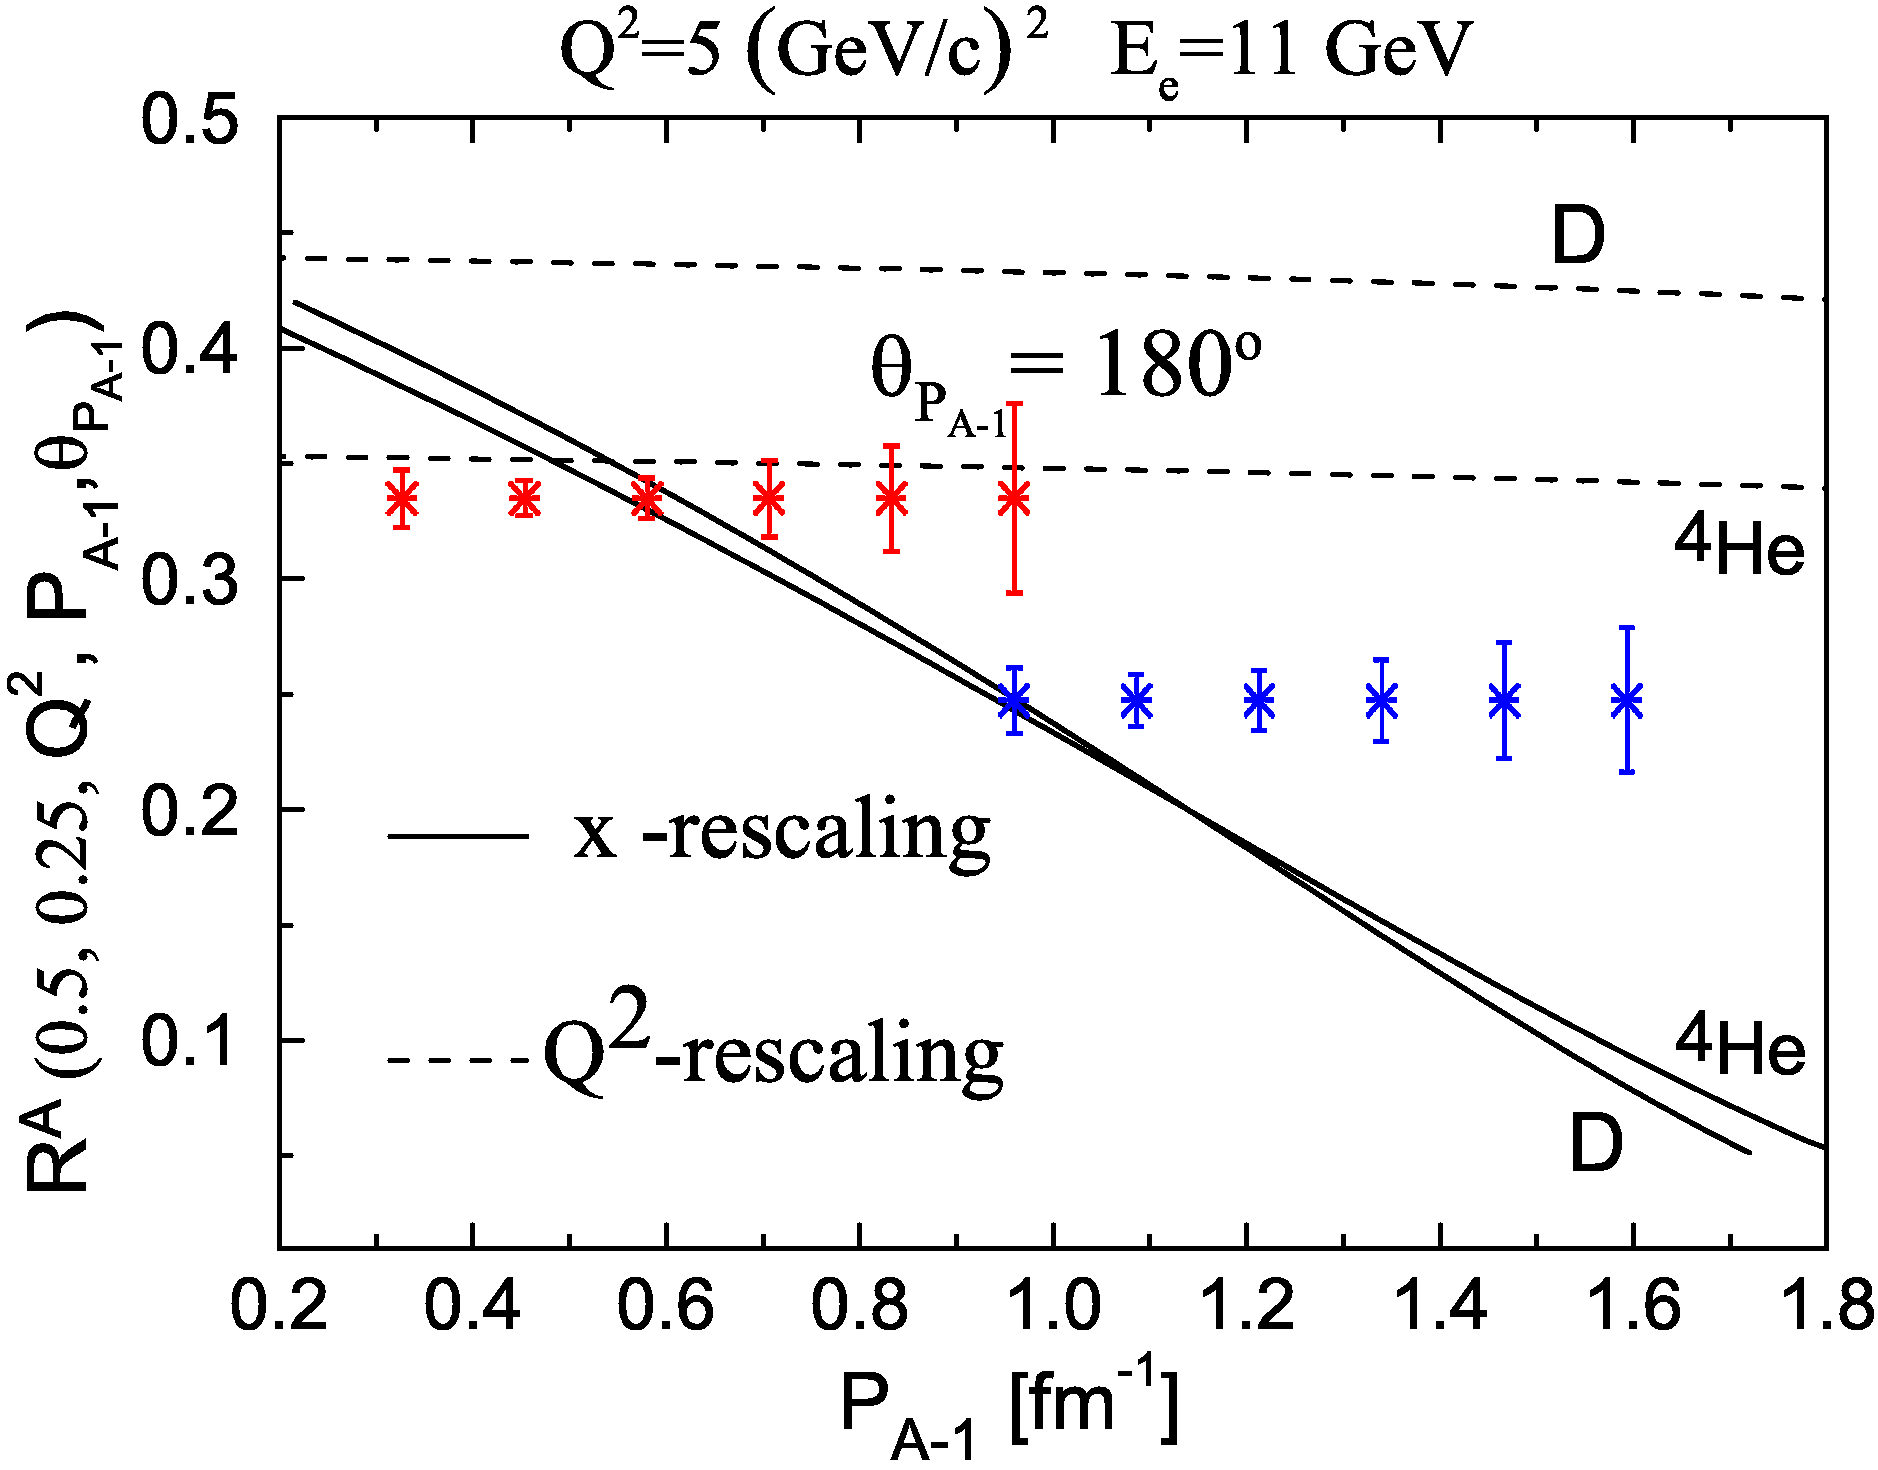
\includegraphics[angle=0, width=0.455\textwidth]{./fig-chap3/Fig5New_180}
    \caption{This figure is similar to figure \ref{fig:ratio_a}, it shows predictions of the ratio $R^A(x,x')$ for $A = 2$ and $A = 4$ as a function of the momentum of the recoil nucleus $A-1$ at perpendicular (left) and backward (right) angle. The full and dashed curves are predictions for CLAS12 kinematic~\cite{CiofidegliAtti1999,CiofidegliAtti2012} of the $x$-rescaling (binding) and $Q^2$-rescaling models, respectively, points are projections for $^2$H (red) and $^4$He (blue).}
    \label{fig:ratio_a_proj}
  \end{center}
\end{figure}

The main goal of our experiment is to discriminate decisively between models of EMC, Fig.~\ref{fig:ratio_a_proj} illustrates this capability. We have here a high differentiation power between x-rescaling and Q$^2$-rescaling models. We note the good coverage and small error bars for $\theta_{P_{A-1}} = 90^\circ$ ($75 < \theta_{P_{A-1}} <105^\circ$), this is due to the better acceptance for this angle. The measurement at backward angle ($\theta_{P_{A-1}} > 150^\circ$), however, is much more difficult and is the main constraint driving our beam time request. Indeed, in order to acceptable error bars and reasonable beam time request, the backward angle are selected up to 150$^\circ$ instead of 160$^\circ$ for the theory prediction.

\subsubsection{Measuring the Local EMC Effect}

\begin{figure}
  \begin{center}
    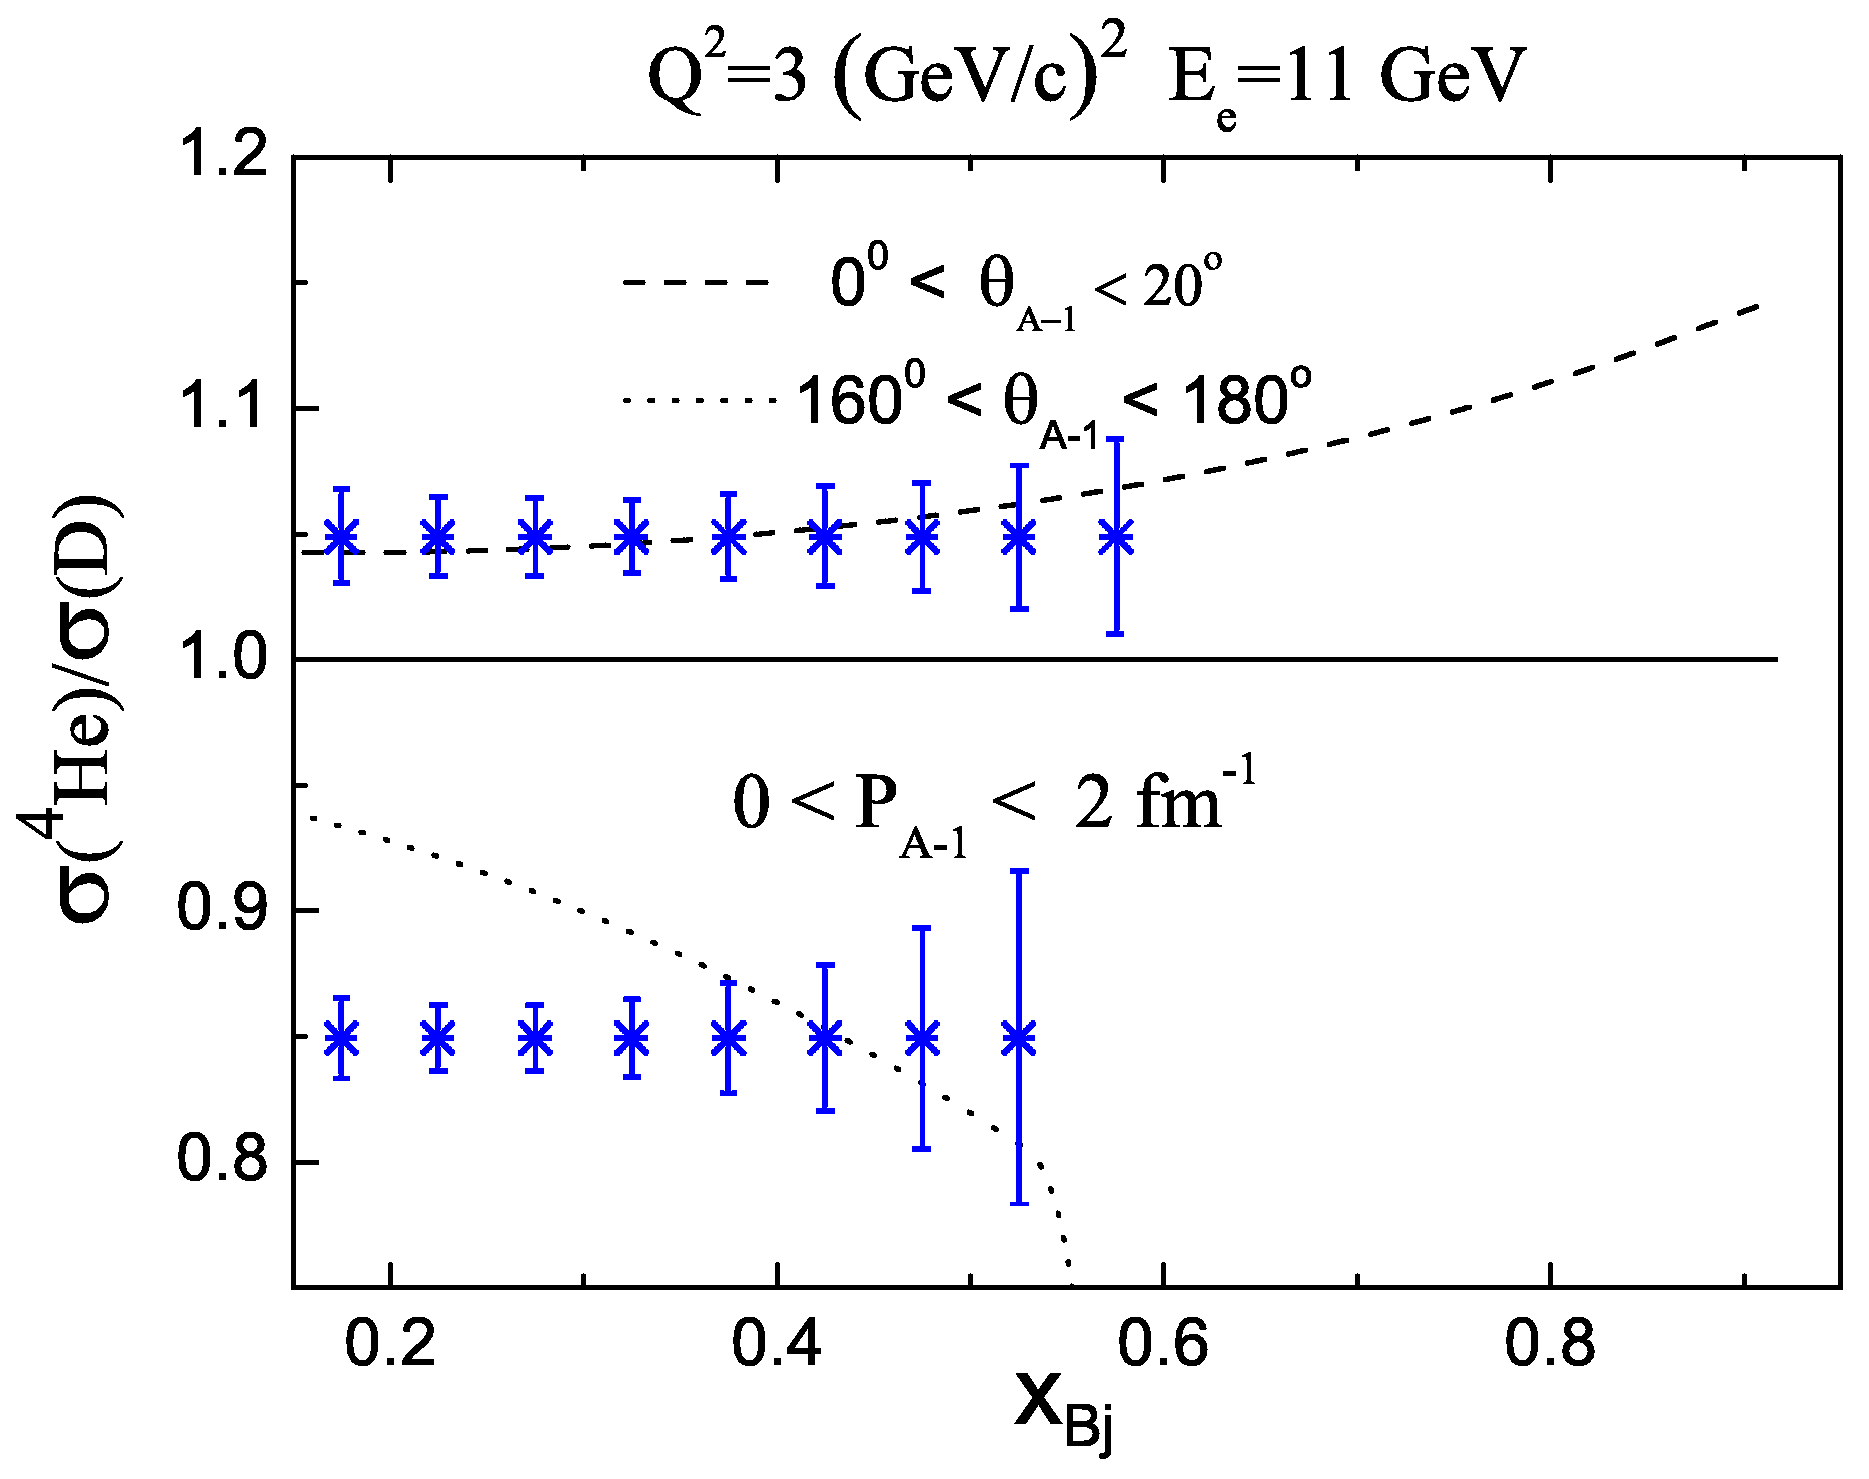
\includegraphics[angle=0, width=0.7\textwidth]{./fig-chap3/Fig10_new}
    \caption{This figure is similar to figure \ref{fig:r0}, it shows the semi-inclusive EMC ratio $R_0(x,Q^2)$ as a function of $x_B$ with recoils emitted forward and backward, the dashed and dotted curves are predictions for the local EMC effect for CLAS12 kinematic~\cite{CiofidegliAtti1999,CiofidegliAtti2012} the blue points are statistical error bar projections for our measurement.}
    \label{fig:fig:r0_proj}
  \end{center}
\end{figure}

The experiment can also confront the striking predictions from the local EMC model for backward versus forward tagged EMC, as illustrated in the Fig.~\ref{fig:fig:r0_proj}. We see that the model prediction will be clearly tested, however the reach in $x_B$ for the backward recoils is also an important constrain on the beam time needed by the experiment. Indeed, the strongest effect is expected at $x_B \sim 0.5$ and necessitates high statistics. 

\subsubsection{Measuring the Flavor Dependent Nuclear Effects}

\begin{figure}
  \begin{center}
    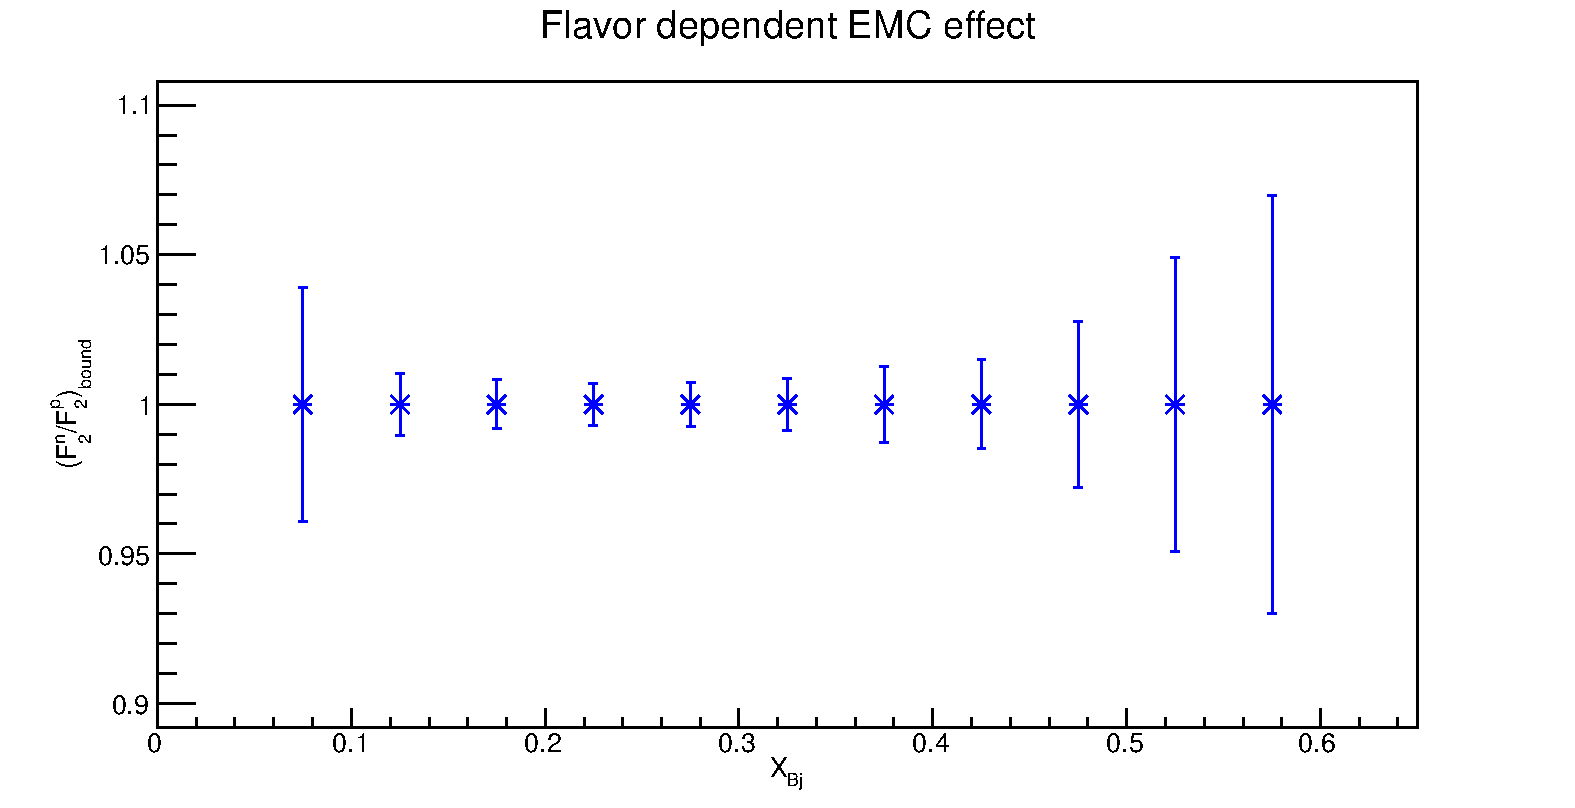
\includegraphics[angle=0, width=0.7\textwidth]{./fig-chap3/flavor}
    \caption{Statistical error bar projections for the ratio $F_2^n/F_2^p$ for bound nucleons as a function of $x_{Bj}$ using an $^4$He target.}
    \label{fig:flavor_proj}
  \end{center}
\end{figure}

Finally with our setup, we can explore the flavor dependence of nuclear PDFs. Figure~\ref{fig:flavor_proj} illustrates our capabilities, theoretical predictions for $^4$He in the isovector model is 1~\cite{Cloet2009}, but others predict that nuclear effects change the d/u ratio and should therefore be observed here~\cite{Brodsky:2004qa}. We will be able to explore any variation in bound nucleons at the 1-2\% level from $x_B$ of $0.1$ to $0.5$.


